\definecolor{cfwone}{HTML}{eef5fa}
\definecolor{cfwtwo}{HTML}{daeaf5}
\definecolor{cfwthree}{HTML}{b2d2e9}
\definecolor{cfwfour}{HTML}{8abbde}

\newcommand{\fwone}[1]{\colbox{cfwone}{#1}\xspace}
\newcommand{\fwtwo}[1]{\colbox{cfwtwo}{#1}\xspace}
\newcommand{\fwthree}[1]{\colbox{cfwthree}{#1}\xspace}
\newcommand{\fwfour}[1]{\colbox{cfwfour}{#1}\xspace}

\newcommand{\fexp}[2]{\texttt{[{\color{darkgray}{#1:#2}}]}\xspace}
\newcommand{\fexptag}[1]{\fexp{TAG}{#1}}
\newcommand{\fexpfrom}[1]{\fexp{FROM}{#1}}
\newcommand{\fexpto}[1]{\fexp{TO}{#1}}
\newcommand{\fexptemp}[1]{\fexp{TEMP}{#1}}


\section{Application 2: Explanations}
\label{sec:app_explain}
%Both counterfactual explanations and semi-counterfactual explanations.
%As defined in \cite{}




\begin{figure}[t]
\centering
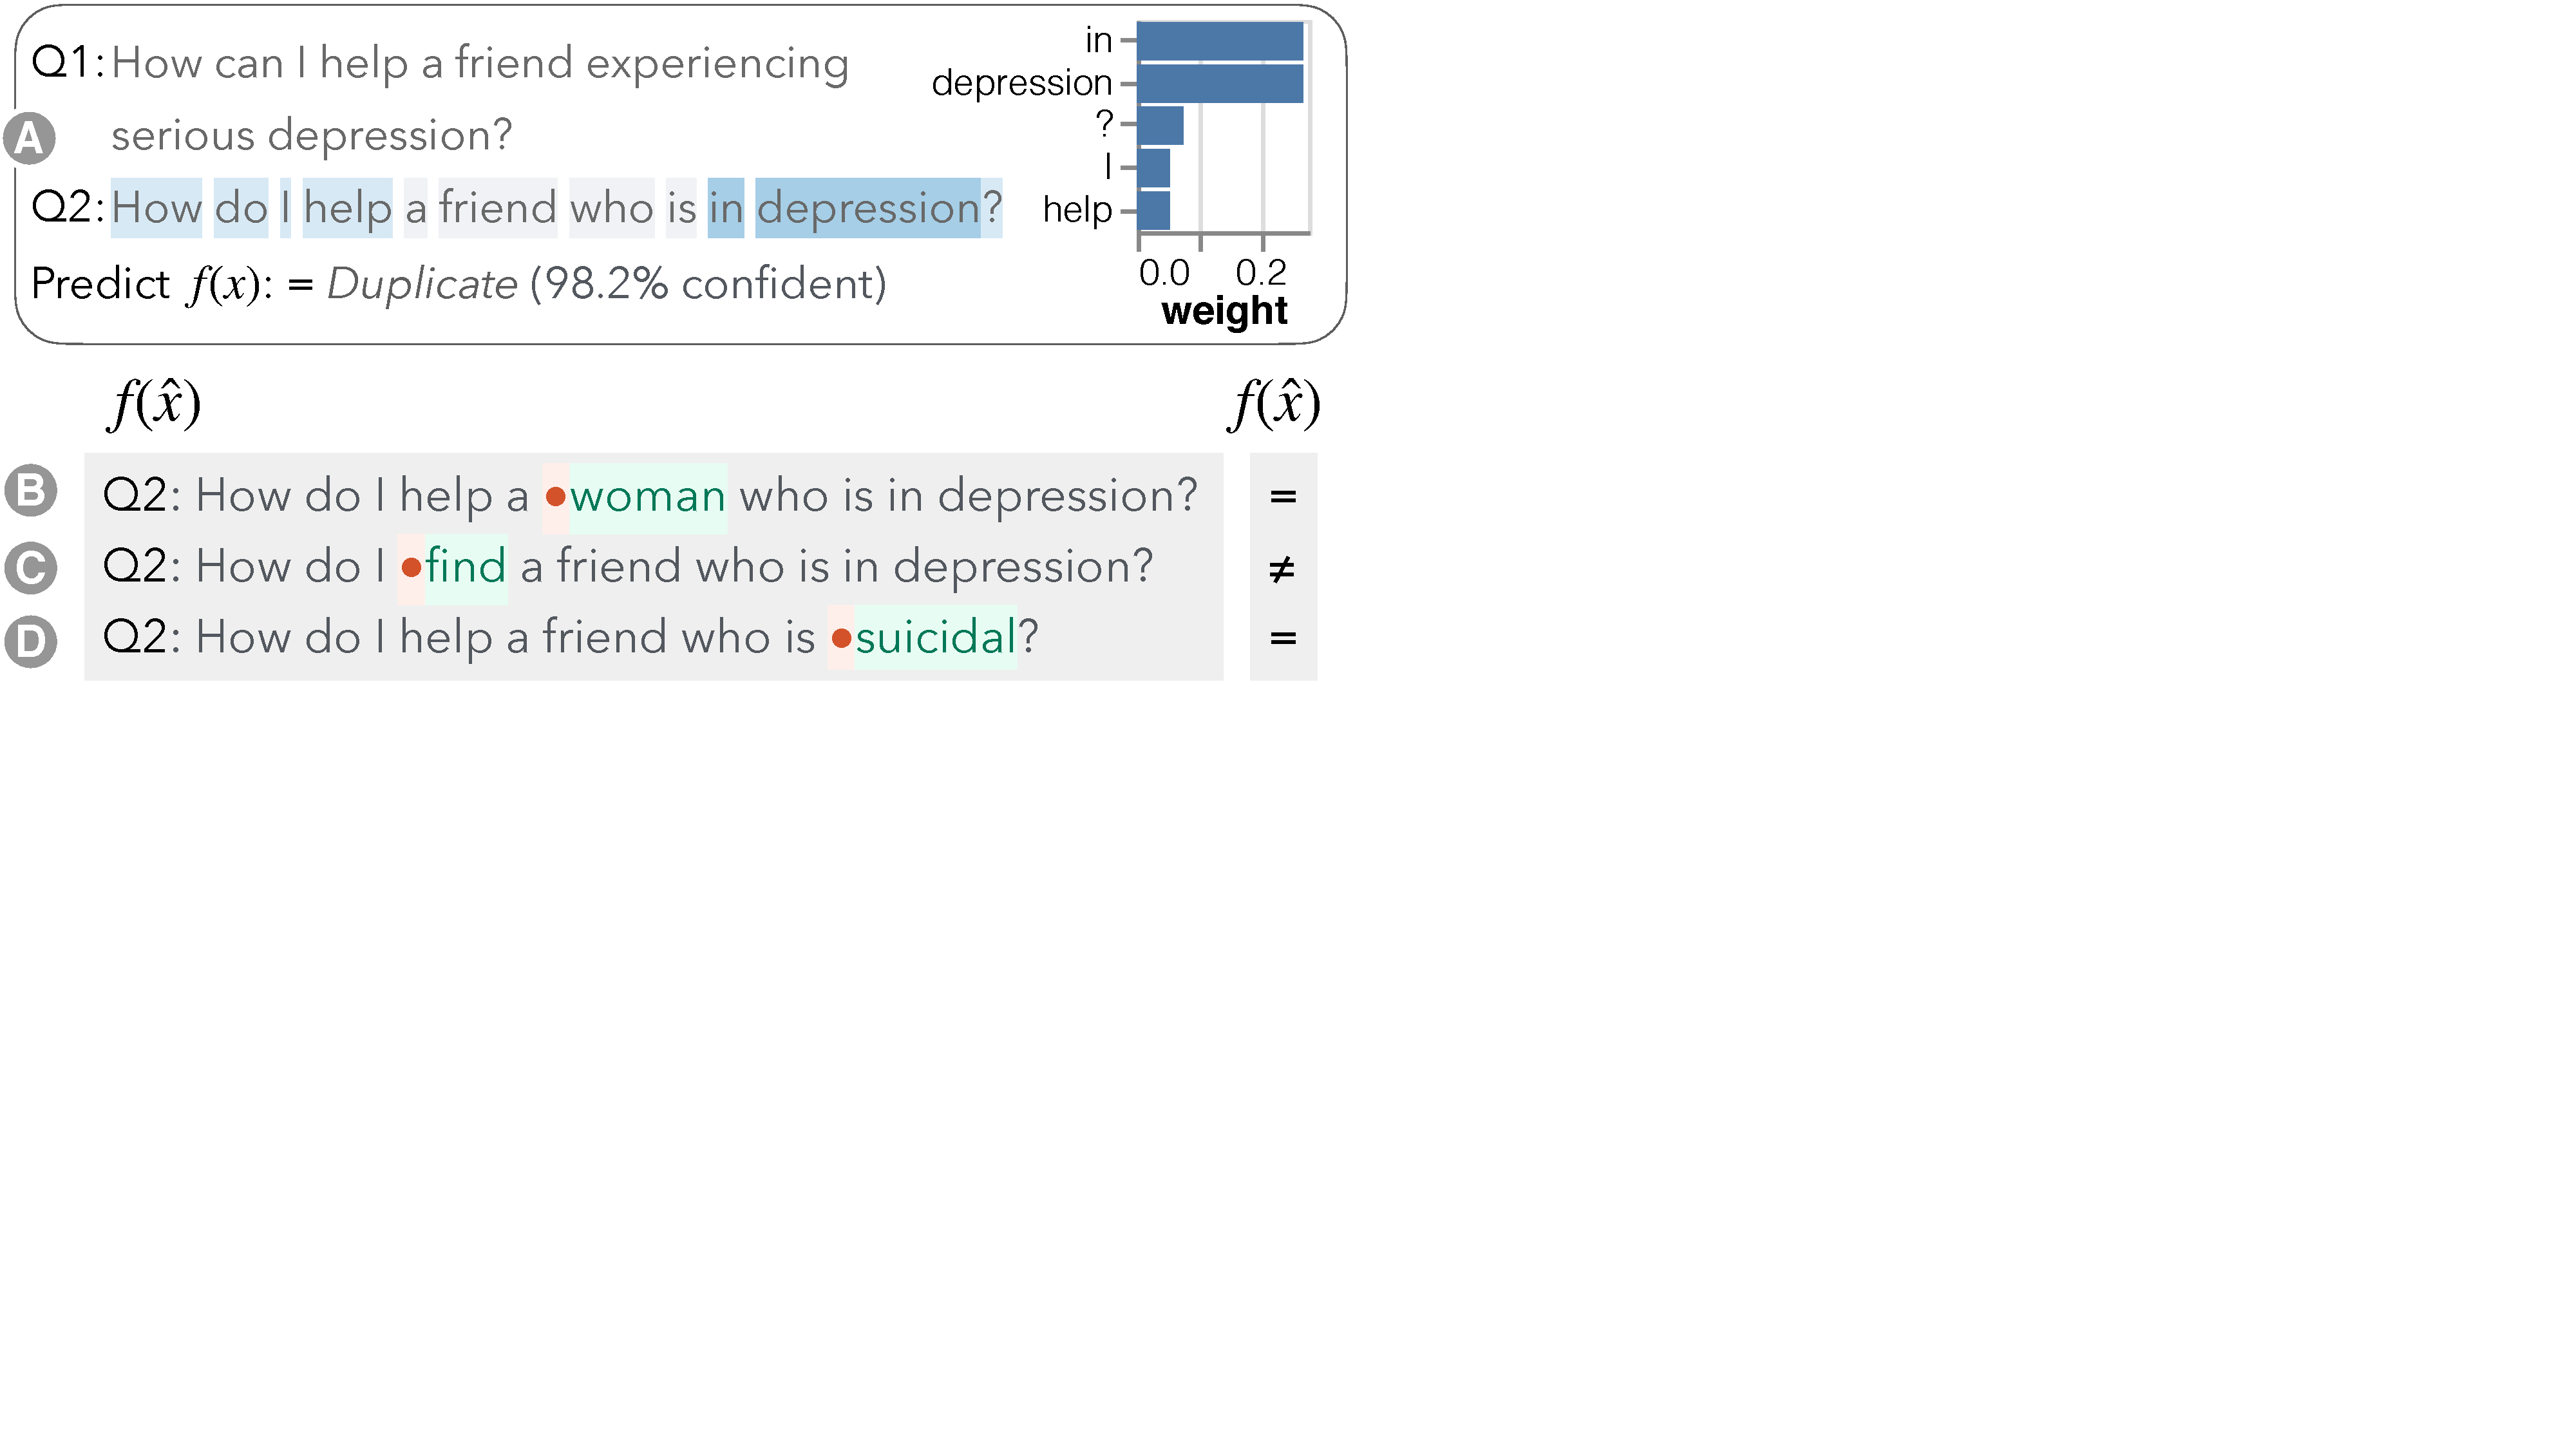
\includegraphics[trim={0 21cm 33cm 0cm},clip,width=1\columnwidth]{figures/explanation_v2.pdf}
\vspace{-15pt}
\caption{
(A) A \qqp instance with its prediction\footnotemark{} showing 98.2\% confidence that the two sentences are duplicative ($=$), as well as the SHAP weights.
%Counterfactual explanations complement SHAP with concrete, readable examples, \eg (C) depicts a surprising flipped prediction ($\neq)$ that was missed by SHAP.
Counterfactual explanations complement SHAP with concrete examples, and alert abnormalities missed by SHAP. \eg (C)
depicts a surprising flipped prediction ($\neq)$.
}
\vspace{-10pt}
\label{fig:explanation}
\end{figure}

%\wts{Finding bugs missed by the feature attribution, and concretizing the opaque weights using readable examples.}
\subsection{Selection: Abnormalities as Explanations}
\label{subsec:local_explain}

\footnotetext{From BERT \qqp model: \url{https://huggingface.co/textattack/bert-base-uncased-QQP}}

Counterfactual explanations have been elusive in NLP, despite being more intuitive than feature attribution methods~\cite{miller}.
Compared to the opaque feature weights in Figure~\ref{fig:explanation}A, Figure~\ref{fig:explanation}B more intuitively shows that the BERT \qqp model considers ``help'' trivial: 
\swap{help}{find} in \emph{Q2} does not change the prediction.
However, conversely, the concrete counterfactuals can be overwhelming, and therefore are less suitable for providing overviews.
Here, we combine the benefits of the two methods, by \emph{augmenting} feature attribution methods (\eg SHAP~\cite{NIPS2017_7062} or LIME~\cite{Ribeiro2016WhySI}) with \emph{abnormal} counterfactuals, which are observed to be more salient~\cite{miller}.
The relationship $\relation{\xp}$ we use for capturing abnormality is the disagreement between \emph{the expected and the actual change of model prediction.}

Given a model $f$, we define the actual prediction change as $\dist(\xp, x)=|\fp(\xp)-\fp(x)|$, where $\fp(x)$ denotes the prediction probability of $f$ on $x$.
Meanwhile, the \emph{expectation} on the prediction change is $\E[\dist(\xp, x)]$, which is the importance (weights) of the perturbed tokens in $x$, estimated by SHAP (details in Appendix~\ref{appendix:exp_rank}).
The mismatch between the reality and the expectation is then:
$$\Delta\dist(\xp, x) = \dist(\xp, x)-\E[\dist(\xp, x)]$$
We select two \emph{expectation violation} counterfactuals:
(1) unexpected large prediction change from trivial perturbations, \ie $\argmax_{\xp} \Delta\dist(\xp, x)$.
In Figure~\ref{fig:explanation}C, \swap{friend}{woman} changes the prediction from \emph{Duplicate} to \emph{Non-Duplicate}, even though ``friend'' is trivial according to SHAP; 
(2) unaffected predictions from large changes, \ie $\argmax_{\xp} -\Delta\dist(\xp, x)$. 
In Figure~\ref{fig:explanation}D, changing the important \remove{in depression} still results in \emph{Duplicate}.

Besides intuitiveness, the selected abnormal $\xp$ additionally highlight a usually overlooked nuance: feature attribution methods estimate weights by \emph{masking} words, and therefore cannot always reflect how models would react to replacements or additions.
Together, we expect them to better calibrate users' trust in the explainer and the predictor.

Note that $\E[\boldsymbol{\cdot}]$ is not necessarily limited to feature attribution.
If we instead use the cosine distance in the latent space~\cite{reimers-2019-sentence-bert}, we may select standalone explanations.
We defer the exploration to future work.


\subsection{Experiment: Counterfactual Simulation}
\label{subsec:exp_user_study}

To verify whether our counterfactual explanations can complement SHAP, we conduct a user study on counterfactual simulation~\cite{hase2020evaluating}, \ie participants predict a model's behavior on $\xp$.
Intuitively, the more they simulate incorrectly, the more information they grasp \emph{if we show the $\xp$}.

%We conduct a user study to verify whether our counterfactual explanations can complement SHAP.
%, as the setup nicely combines the overview provided by SHAP, and the decision boundaries it omits.
%\footnote{We defer more sophisticated designs and evaluations for interactive and global explanation to future work.}
%, where participants are asked to predict model's behavior on the given variations of a base example.
%The study takes the form of counterfactual simulation~\cite{hase2020evaluating}, with participants predicting a model's behavior on $\xp$.
%Intuitively, the more they simulate incorrectly, the more information they grasp \emph{if we show the counterfactuals}.

\paragraph{Procedure.}
We recruited 13 graduate students who have intermediate NLP knowledge and have experience using model explanations, and asked them to simulate the aforementioned \qqp model for 20 rounds.
In each round, the participants were given a base example with the model's prediction, as well as the SHAP weights, highlighted in the text and with a bar chart (Figure~\ref{fig:explanation}A).
Moreover, they could create up to 10 counterfactuals on their own, and query the model predictions on them (they used around 6 chances.)
%More interactions with the predictor usually result in better mental models~\cite{miller}, and we are interested in whether our counterfactuals \emph{still add information} after sufficient interactions (they usually used 6 chances.)
Participants then simulated the model's predictions on six given counterfactuals, two from each of the following three conditions.
We concluded the study with surveys on their counterfactual creation and simulation strategies.
%The interface is in Appendix~\ref{appendix:exp_user_study}.

%We validate this hypothesis in user study, where expert users did slightly better than random (accuracy: $55 \pm 6\%$) at predicting what a model would do on \sysname counterfactuals, even after seeing SHAP explanations \cite{NIPS2017_7062} and manually creating counterfactuals to explore the model's behavior. This indicates that seeing such explanations would add a lot of information that users are currently missing (much of which consisting of mistaken model predictions) even if when they perform manual counterfactual analysis and use feature attribution methods.


\newcommand{\cshap}{\emph{SHAP-c}\xspace}
\newcommand{\crandom}{\emph{Random}\xspace}
\newcommand{\chuman}{\emph{Human}\xspace}
\paragraph{Conditions.} 
We compare three types of counterfactuals:
(1) \cshap, the \sysname-generated counterfactuals, selected to complement SHAP; 
(2) \crandom, the randomly selected \sysname counterfactuals; 
(3) \chuman, the human-generated counterfactuals, in which two graduate students (not participants) played with the model, and each created one $\xp$ where the prediction was incorrect and counterintuitive according to the SHAP score on $x$.
The authors manually checked that all counterfactuals were fluent and unambiguous.

\begin{comment}
\begin{figure}[t]
\centering
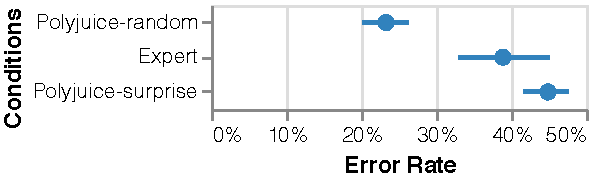
\includegraphics[width=1\columnwidth]{figures/err_rate.pdf}
\vspace{-15pt}
\caption{
Error rates on counterfactuals in different conditions. The higher the error rate, the more information missed by the participants, therefore can better complement manual counterfactual analysis and SHAP.
}
\vspace{-10pt}
\label{fig:err_rate}
\end{figure}
\end{comment}

\paragraph{Results.}
As a within-subject study, we compared \emph{the error rate of human simulations across the three conditions}.
%As in Figure~\ref{fig:err_rate}, 
Participants were able to simulate the cases in \crandom (error rate $e=23\%\pm6\%$), possibly because they contained more minor variations that aligned with participants' mental models built on the the SHAP values and their interactions with the models~\cite{miller}.
They missed more \chuman ($e=39\%\pm11\%$) cases, and were even worse on \cshap ($45\%\pm 6\%$, only slightly better than random guess).%, though the confidence intervals overlap.
This shows that \cshap counterfactuals are beyond participants' learnings from feature attributions and manual counterfactual analysis, and \emph{would still add value if they were presented.}
They are also at least as effective as the \chuman ones, which is very expensive to create --- each graduate student spent 1.5--2 hours to generate 20 ``abnormal'' counterfactuals.

Usually, participants simulated the model incorrectly because they missed the inspection spots.
For example, they repeatedly perturbed ``depression'' in Figure~\ref{fig:explanation}A, and therefore had to guess when simulating Figure~\ref{fig:explanation}B.
However, in 24\% of the missed \cshap cases, participants successfully covered the related pattern,\footnote{At least one of their queries perturbed the same spans as $\xp$, and query text overlaps with the $\xp$ for over 70\%.} but were misled by their inspections --- ``followed similar examples I tried,'' as one subject articulated.
It was hard for them to imagine the model predicting \emph{Duplicate} on Figure~\ref{fig:explanation}B (\swap{help}{find}), when it predicted \emph{Non-Duplicate} on their query \exinline{How do I \swap{help}{play with}...?}
The number dropped to $15\%$ for the \chuman condition.
In other words, \emph{\cshap found more bugs within spots where humans considered inspected.}
%\hao{this is very interesting. close by summarizing the conclusion?}


\paragraph{Takeaways.}
\sysname counterfactuals complement feature attribution methods and counterfactual analysis, as effectively as hiring a second expert for the analysis (but much cheaper).
In particular, they highlight erroneous spots where humans may be misled by their own analysis.
